\section{\uppercase{Experimental results}}\label{sec:results}

\subsection{Encoder Evaluation by Modality}

\noindent
Each encoder is first measured against its field's standard benchmark, so any
later fusion result rests on encoders already tested in isolation.
Table~\ref{tab:perleg} collects both comparisons.

On UJIIndoorLoc, WiFi-Net reaches an MAE of $8.69$~m on the validation scans,
against $15.17$~m for wlan\_localization\footnote{The $7.9$~m error in Section~\ref{sec:related} is the original 1-NN result on UJIIndoorLoc; wlan\_localization is an open-source $k$-nearest-neighbor implementation ($k=3$, distance-weighted) evaluated here on the validation split.}, a reduction of $42.7\%$. The benchmark
fixes $520$ access points and carries no trajectory structure, so the comparison
isolates the mapping from fingerprint to position with no temporal context.

The inertial comparison is more demanding. On RoNIN canonical, IMU-CNN attains a
raw ATE of $9.72$~m on the $32$ sequences held out from training, against
$5.14$~m for ResNet1D, trailing by $89.2\%$. The encoders differ sharply in size:
IMU-CNN holds about $0.05$~M parameters against ResNet1D's $4.6$~M, a factor of
roughly $95$. IMU-CNN is competitive within its own domain but pays a cross-subject
generalization cost, which it incurs on a significantly smaller budget. The drift is visible
on one such sequence in Figure~\ref{fig:ronin_traj}.

The aggregate figure hides a more even picture sequence by sequence.
Figure~\ref{fig:ronin_perseq} ranks IMU-CNN's five best sequences by raw
ATE against the ResNet1D mean of $5.14$~m: four fall below that mean. The $89.2\%$
gap thus comes from a few harder sequences, not a uniform shortfall.

\begin{table}[tb]
\caption{Encoder evaluation by modality, each encoder scored on its field's
  standard benchmark (MAE on UJIIndoorLoc, raw ATE on RoNIN canonical); the
  reference is wlan\_localization for UJIIndoorLoc and ResNet1D for RoNIN
  canonical. Bold marks the lowest error in each row.}\label{tab:perleg}
\centering
\footnotesize
\setlength{\tabcolsep}{2pt}
\begin{tabular}{|l|l|c|c|c|}\hline
Benchmark & Metric & Reference & Ours & Rel.\ $\Delta$ \\ \hline
UJIIndoorLoc (val) & MAE & 15.17 & \textbf{8.69} & $-42.7\%$ \\ \hline
RoNIN canonical & raw ATE & \textbf{5.14} & 9.72 & $+89.2\%$ \\ \hline
\end{tabular}
\end{table}

\begin{figure}[tb]\centering
  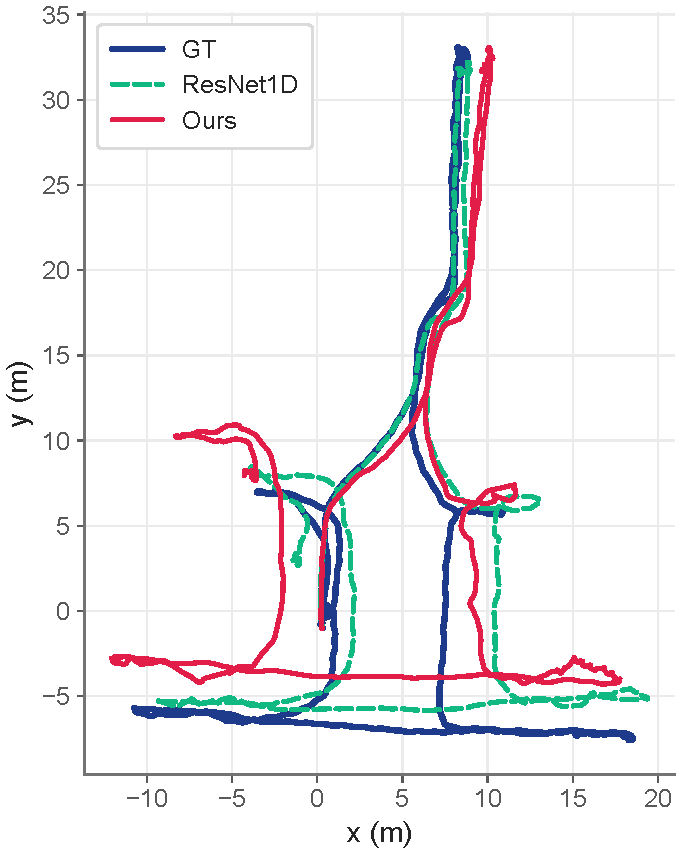
\includegraphics[width=1\columnwidth]{figures/fig_ronin_traj.pdf}
  \caption{RoNIN canonical held-out sequence: ground truth, ResNet1D, and
    IMU-CNN (ours). The lighter inertial encoder follows the route but
    accumulates more drift than ResNet1D.}\label{fig:ronin_traj}
\end{figure}

\begin{figure}[tb]\centering
  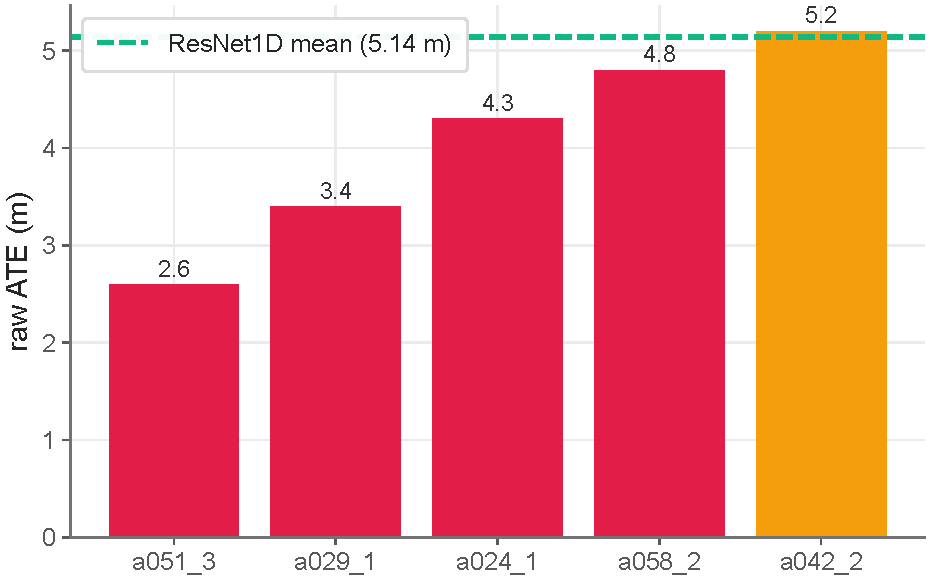
\includegraphics[width=1\columnwidth]{figures/fig_ronin_perseq.pdf}
  \caption{IMU-CNN's five best RoNIN canonical sequences by raw ATE, against the
    dashed ResNet1D mean of $5.14$~m. Four of the five fall below that mean, so
    the encoder is competitive per sequence despite trailing on the aggregate.}
  \label{fig:ronin_perseq}
\end{figure}

\subsection{End-to-End Fusion}

\begin{figure*}[t!]\centering
  \begin{subfigure}[t]{0.45\textwidth}\centering
    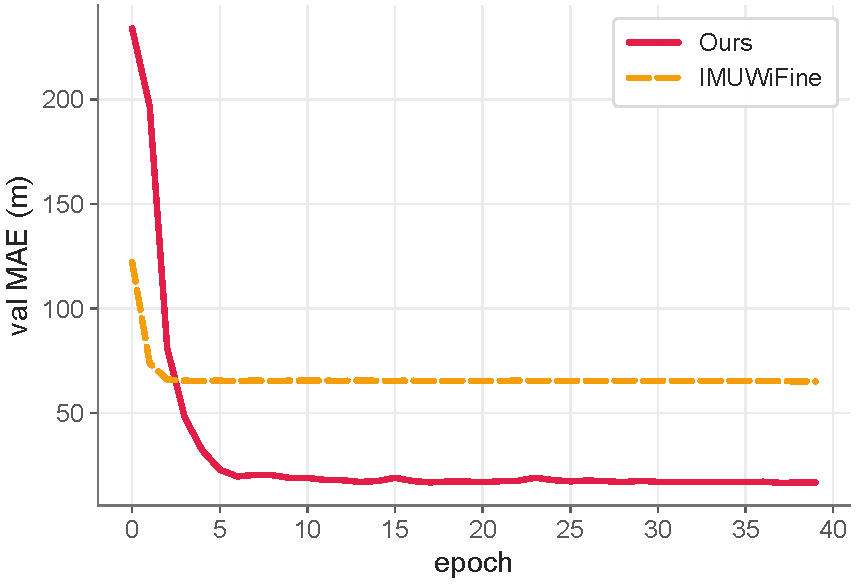
\includegraphics[width=\linewidth]{figures/fig_msiln_curves.pdf}
    \caption{Validation MAE over training. The proposed model converges toward
      roughly $16$~m, while the IMUWiFine LSTM plateaus near $65$~m.}
    \label{fig:msiln_curves}
  \end{subfigure}\hfill
  \begin{subfigure}[t]{0.45\textwidth}\centering
    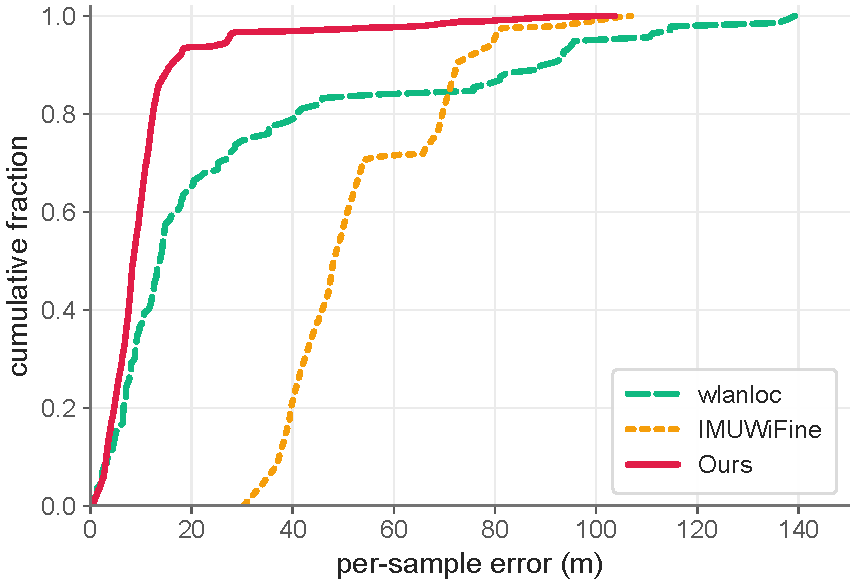
\includegraphics[width=\linewidth]{figures/fig_msiln_cdf.pdf}
    \caption{Error distribution per sample on the test session. The proposed
      method reaches $90\%$ of samples within roughly $15$~m.}
    \label{fig:msiln_cdf}
  \end{subfigure}\hfill
  \begin{subfigure}[t]{0.45\textwidth}\centering
    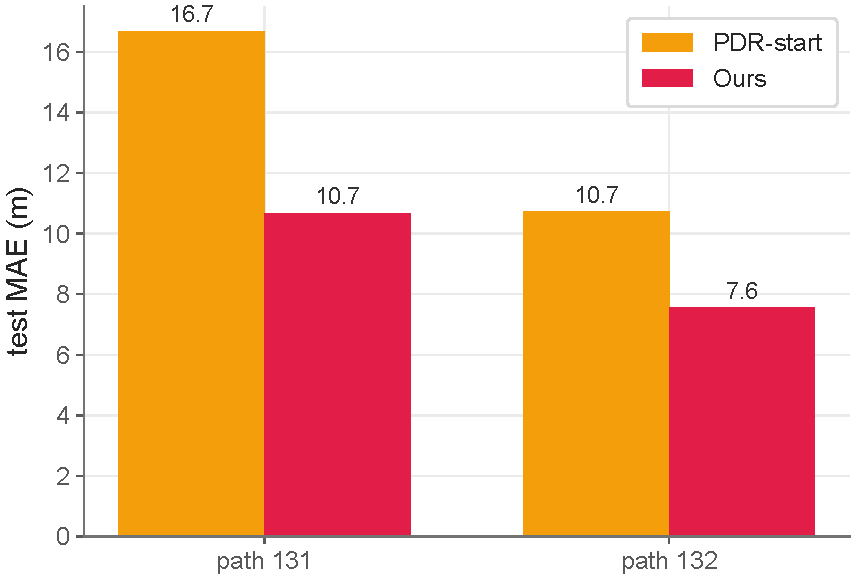
\includegraphics[width=\linewidth]{figures/fig_msiln_perpath.pdf}
    \caption{Test MAE for each of the two paths where the proposed method is ahead
      of PDR-from-start.}
    \label{fig:msiln_perpath}
  \end{subfigure}
  \caption{MSILN site1/B1 fusion across sessions. (\subref{fig:msiln_curves})
    training convergence against the IMUWiFine LSTM, (\subref{fig:msiln_cdf})
    test error distribution per sample against wlan\_localization and
    IMUWiFine, and (\subref{fig:msiln_perpath}) MAE per path against
    PDR-from-start on the paths where the proposed method is ahead.}
  \label{fig:msiln}
\end{figure*}

\noindent
With both encoders validated, the set transformer fuses them, evaluated first in
the controlled simulation, then on the real collection across sessions that
carries the headline claim. Table~\ref{tab:fusion} collects the fusion results
against the three named reference methods.

In the Webots simulation the WiFi field is clean by construction. There the
model fusing the two modalities at $K=4$ reaches $0.61$~m MAE on test
(Figure~\ref{fig:webots_scatter}). This figure, below one meter, is a controlled
reference point, not a deployment claim: with a synthesized WiFi field it is not
directly comparable to the real numbers below.

MSILN site1/B1 supplies the real evaluation across sessions. On the test session,
held out for evaluation, the set transformer reaches $10.90$~m MAE, against
$28.31$~m for wlan\_localization, $12.49$~m for PDR-from-start and $52.69$~m for
IMUWiFine. On the
validation session the margin is narrow: $16.67$~m against $16.88$~m for
PDR-from-start, with wlan\_localization at $21.26$~m and IMUWiFine at $65.15$~m.
Where wlan\_localization nearly doubles its error from validation to test, the
fusion error falls. Fusing the dense inertial stream against the sparse absolute
reference maintains position across the session boundary. IMUWiFine, itself a learned
WiFi--IMU fusion, remains above $52$~m on both splits
(Figure~\ref{fig:msiln_curves}), an informative negative result for learned fusion
under fingerprint drift. Beating wlan\_localization, a distance-weighted WiFi
$k$-NN with no motion model, is expected of any method that tracks motion, so the
$-61.5\%$ figure is a sanity check; the comparisons that carry weight are against
PDR-from-start and the IMUWiFine LSTM. The full distribution of test error per
sample is in Figure~\ref{fig:msiln_cdf}, and error for each path against
PDR-from-start on the two paths where the proposed method is ahead in
Figure~\ref{fig:msiln_perpath}.




\begin{table*}[tb]
\caption{End-to-end fusion: position MAE (m). The simulation has no public
  reference fusing two modalities; the MSILN comparison runs across sessions
  against three named reference methods. Bold marks the lowest error in each
  row.}\label{tab:fusion}
\centering
\begin{tabular}{|l|c|c|c|c|}\hline
Dataset (split) & wlan\_localization & PDR-from-start & IMUWiFine & Ours \\ \hline
Webots sim (test) & n/a & n/a & n/a & \textbf{0.61} \\ \hline
MSILN site1/B1 (val) & 21.26 & 16.88 & 65.15 & \textbf{16.67} \\ \hline
MSILN site1/B1 (test) & 28.31 & 12.49 & 52.69 & \textbf{10.90} \\ \hline
\end{tabular}
\end{table*}



\begin{figure}[!hb]\centering
  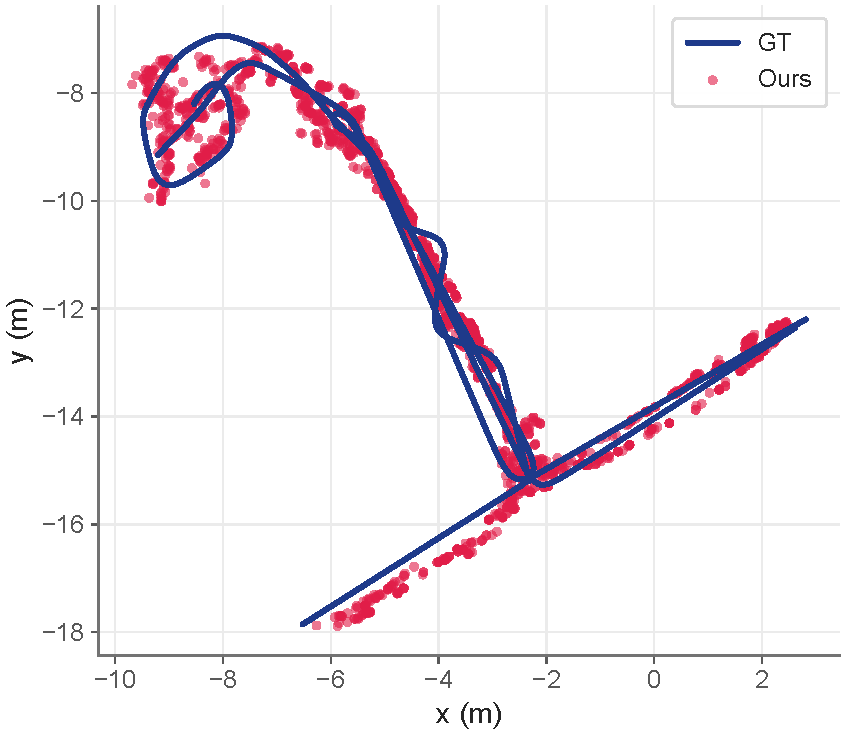
\includegraphics[width=1\columnwidth]{figures/fig_webots_scatter.pdf}
  \caption{Webots simulation test paths: predicted positions (ours) against
    ground truth. The controlled lab admits tracking below one meter when the WiFi
    field is clean.}\label{fig:webots_scatter}
\end{figure}

\subsection{Generalization to a Further Dataset}

\noindent
IMUWiFine floor~4~\cite{nurpeiissov2022imuwifine} provides the complementary test:
a split that holds out paths within the same distribution, on the LSTM's own
dataset, where the proposed method gains nothing from session drift. It reaches a
test MAE of $6.37$~m on this split, against a validation MAE of $2.31$~m.

On four paths where the proposed method is best or competitive
(Figure~\ref{fig:iwfine_showcase}), the LSTM tracks its home ground to roughly one
meter, and the proposed method takes two of them (path~$69$ at $0.93$~m and
path~$64$ at $0.73$~m) while trailing narrowly on the others. Both learned methods
improve over wlan\_localization by roughly two to three times on every path. The
LSTM is therefore strong within its own distribution but not across sessions,
whereas the proposed method is competitive within distribution and holds up on the
MSILN test across sessions.

\begin{figure}[!hb]\centering
  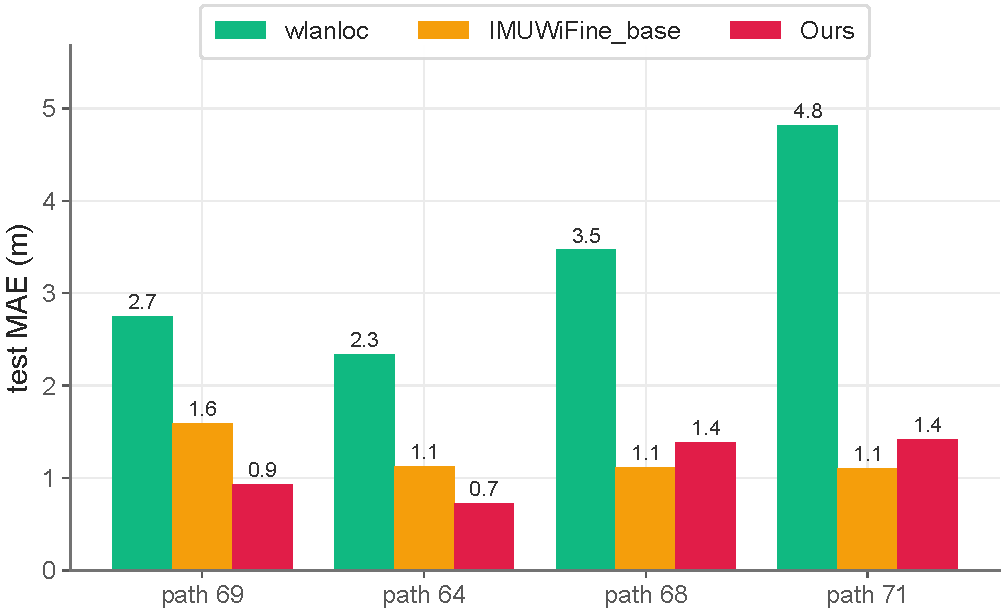
\includegraphics[width=1\columnwidth]{figures/fig_iwfine_showcase.pdf}
  \caption{IMUWiFine floor~4: test MAE (m) for each of four paths where the proposed
    method is best or competitive.}\label{fig:iwfine_showcase}
\end{figure}

\subsection{Robustness and Ablations}

\noindent
The remaining experiments run on the Webots simulation, where every signal is
controlled and individual sensors can be suppressed or aged on demand, realizing
the missing ($a_i=0$) and stale (large $|\Delta t_i|$) conditions defined in
Section~\ref{sec:problem}.

\textbf{Modality dropout.} Suppressing a modality at test time exposes what each
stream contributes. With WiFi only the test MAE is $0.86$~m; with IMU only it is
$3.50$~m; with both it is $0.61$~m. The WiFi token provides the absolute
reference, so dropping IMU costs little, while IMU alone drifts without it.

\textbf{Staleness.} Aging the WiFi token while the IMU stream stays fresh exposes
the cost of delayed measurements. The test MAE climbs gradually,
$0.61 \to 1.13 \to 1.48 \to 1.84 \to 2.05$~m, reaching the level of IMU alone at
$3.50$~m only once the reference is fully stale: a slope rather than a cliff across
moderate delays.

\textbf{Latency.} On the Quadro P4000 the model runs at $4.77$~ms per sample at
batch size $1$ and $0.146$~ms at batch size $32$, fast enough for real-time use.

\subsection{Limitations}

\noindent
Two limitations qualify the results. First, the $+89.2\%$ inertial gap on RoNIN
canonical persists under Umeyama alignment~\cite{umeyama1991}, narrowing only to
$+48.2\%$ ($7.62$~m versus ResNet1D's $5.14$~m).
Second, the MSILN test split is dominated by one WiFi dense path of $786$ samples,
roughly $28\%$ of the test mass, so the test figure is best read alongside the
validation figure rather than in isolation.
